% Chapter 4

\chapter{Experimental results} % Main chapter title

\label{Chapter4} % For referencing the chapter elsewhere, use \ref{Chapter1} 

\lhead{Chapter 4. \emph{Experimental results}} % This is for the header on each page - perhaps a shortened title

%----------------------------------------------------------------------------------------

\section{Data Generation}

\subsection{Building training and testing dataset}
We downloaded viruses, bacteria and archaea genomes from RefSeq database then we divided them randomly into a train and test genomes with 80\% of total base pairs in training. Table \ref{table:genome_stats} shows the number of genomes we used in training and testing. We processed all available viral genomes until Nov. 1, 2017 and a sample from prokaryotic genomes due to the huge number of available prokaryotic genomes. Then, we converted the viral genomes into non-overlapping fragments of different lengths n = \{100, 500, 1000, 3000\}. We generated an approximate number of non-overlapping fragments of prokaryotic genomes with the same lengths randomly as well. (Table \ref{table:fragments_stats}). We balanced the data of both classes using random under-sampling technique to avoid the bias to the majority class with the deep neural network. Figure \ref{fig:data_pipline} shows more details for data pipeline.

\begin{figure}[!htbp]
	\centering
	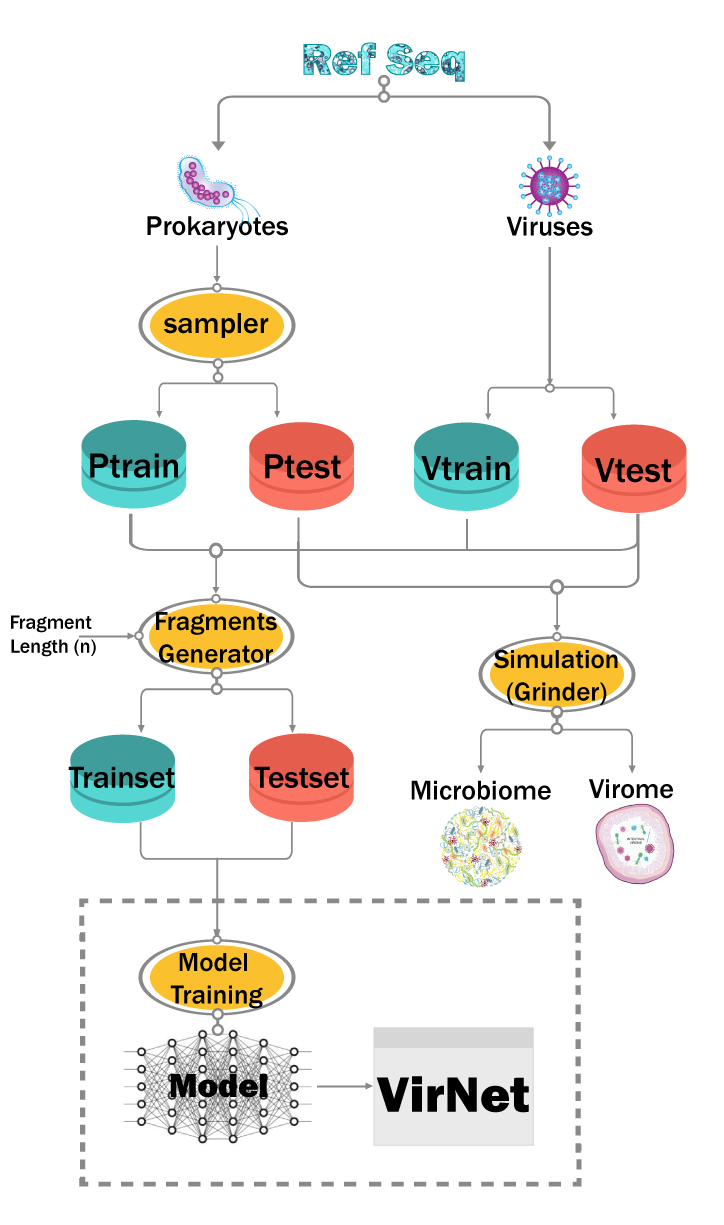
\includegraphics[width=\columnwidth]{Pictures/data_pipeline.PNG}
	\caption{VirNet Data Pipeline}
	\label{fig:data_pipline}
\end{figure}

\begin{table}[!htbp]
	\centering
	\begin{tabular}{||c c c c||} 
		Genome & Train & Test & Total \\ [0.5ex] 
		\hline\hline
		Viruses & 7686  & 1870 & 9556 \\ 
		Prokaryotes & 143241  & 35543 & 178784  \\ [1ex] 
	\end{tabular}
	\caption{The number of used genomes from RefSeq}
	\label{table:genome_stats}
\end{table}

\begin{table}[h!]
	\centering
	\begin{tabular}{||c c c||} 
		Fragment Length (N) & Train & Test \\ [0.5ex] 
		\hline\hline
		100 bp & 2088863  & 527020  \\ 
		500 bp & 420857  & 106168  \\
		1000 bp & 212253  & 53528  \\
		3000 bp & 73163  & 18425  \\ [1ex] 
	\end{tabular}
	\caption{The number of fragments generated from viruses genomes}
	\label{table:fragments_stats}
\end{table}

\subsection{Generating simulated virome and microbiome}
Grinder \cite{angly2012grinder} is an open-source tool commonly used for generating a simulate amplicon and shotgun metagenomic datasets from reference genomes. 
We generated two metagenomic data of virome and microbiome of 1M reads and fragment length 100bp using Grinder with our reference test genomes to simulate shotgun metagenomic sequences in order to verify the ability of our tool to detect viral reads in metagenomic data instead of generated fragments from the reference genomes. The virome data has 75\% of viral reads while microbiome has 25\%. Moreover, we used Illumina error model indicated by mutation\_dist poly4 3e-3 3.3e-8 and mutation ratio 91:9 (9 indels for each 91 substitution mutations) because for Illumina indel errors occur more often than substitution errors \cite{laehnemann2015denoising}. Table \ref{table:simulate_stats} shows simulated data statistics.  \\

\begin{table}[!htbp]
	\centering
	\begin{tabular}{||c c c||} 
		& Microbiome & Virome \\ [0.5ex] 
		\hline\hline
		Bacteria Length & 75450367  bp  & 17551396 bp  \\
		Bacteria Genomes & 1488 & 422\\
		Bacterial reads & 803742 & 176059\\
		Viruses Length & 25133078 bp  & 52609236 bp  \\ 
		Viruses Genomes & 845 & 1870\\
		Viral reads & 196258 & 823941 \\  
		Viral Ratio & 25.00\% & 75.00\% \\ 
		Library coverage &  0.994x &  1.001x  \\
		Diversity (richness) & 2302 & 2726 \\ [1ex]
	\end{tabular}
	\caption{Grinder Simulated Metagenome}
	\label{table:simulate_stats}
\end{table}


\subsection{Case Study: Real metagenomic data}
We applied our tool to two real metagenomes as a case study
\begin{enumerate}
	\item \textbf{454}: Subtropical freshwater microbial and viral metagenome (SRR648314).\
	\item \textbf{Illumina}: Lake Michigan virome (SRX995836).
\end{enumerate}
Our tool is able to read not only fasta files and fastq files. Furthermore, it is able to deal with paired-end reads i.e. if one of the two pairs is identified as a virus, the other should be the same. If there are conflicts between the classifications of the two pairs; this pair could be denoted as ambiguous.

\section{Results}
\subsection{Results for generated fragments}
We tested VirNet on different lengths of fragments n= \{100, 500, 1000, 3000\} from our testing set of viruses and prokaryotes RefSeq genomes. Moreover, we compared the output results to VirFinder results on the same training and testing data. VirNet predictions outperformed VirFinder for fragments with length 500, 1000 and 3000 (Figure \ref{fig:accuracy_graph}). The model reached to 82.82\% of accuracy whereas VirFinder tool obtained 75.61\%. Moreover, VirFinder can perdict the short fragments with length 100. Figures \ref{fig:roc_auc_virfindera} and \ref{fig:roc_auc_virneta} shows ROC-AUC curves of both tools on the testing set. Table \ref{table:virfinder_results} shows the comparison between both tools in terms of accuracy, average precision and average recall.

%\begin{table}[h!]
%	\centering
%	\begin{tabular}{||c l l l l l l l l||} 
%		Length(N) &	\multicolumn{2}{l}{Accuracy} & \multicolumn{2}{l}{Avg. Precision} & \multicolumn{2}{l}{Avg. Recall} &	\multicolumn{2}{l}{ROC-AUC} \\ [0.5ex] 
%		& VirNet & VirFinder & VirNet & VirFinder & VirNet & VirFinder & VirNet & VirFinder \\
%				\hline\hline
%		100 & 71.29\% &	63.9\%	& 0.72 & 0.64 & 0.71 & 0.64 & 0.80 & 0.64 \\
%		500 & 82.82\% &	75.61\% & 0.83 &	0.76 & 0.83 & 0.76 & 0.9 & 0.75 \\
%		1000 & 86.82\% &	80.28\% &  0.87 & 0.82 & 0.87 & 0.80 & 0.93 & 0.78 \\
%		3000 & 90.10\% &	87.11\% & 0.91 & 0.88 & 0.90 & 0.87 & 0.94 & 0.83\\[1ex]
%	\end{tabular}
%	\caption{VirFinder Results on our test-set}
%	\label{table:virfinder_results}
%\end{table}

\begin{table}[!htbp]
	\centering
	\begin{tabular}{||c l l l l l l||} 
		Length(N) &	\multicolumn{2}{l}{Accuracy} & \multicolumn{2}{l}{Avg. Precision} & \multicolumn{2}{l}{Avg. Recall}\\ [0.5ex] 
		& VirNet & VirFinder & VirNet & VirFinder & VirNet & VirFinder \\
		\hline\hline
		100 & 71.29\% &	63.9\%	& 0.72 & 0.64 & 0.71 & 0.64 \\
		500 & 82.82\% &	75.61\% & 0.83 &	0.76 & 0.83 & 0.76\\
		1000 & 86.82\% &	80.28\% &  0.87 & 0.82 & 0.87 & 0.80 \\
		3000 & 90.10\% &	87.11\% & 0.91 & 0.88 & 0.90 & 0.87 \\[1ex]
	\end{tabular}
	\caption{Comparison on fragments test-set}
	\label{table:virfinder_results}
\end{table}

\subsection{Results for simulated metagenomes}

As mentioned before, we tested VirNet on a simulated metagenomes of 100 bp and we found that VirNet performed much better than VirFinder. VirNet shows accuracy is 71.3\% on the virome data and 72.14\% on the microbiome data while VirFinder is 62.77\% on the virome data and 64.49\% on the microbiome data Table \ref{table:virfinder_results_simulated}). The ROC-AUC curves of both tools shows the difference between them (Figures \ref{fig:roc_auc_virfinderb} and \ref{fig:roc_auc_virnetb}).

\begin{figure}
	\centering
	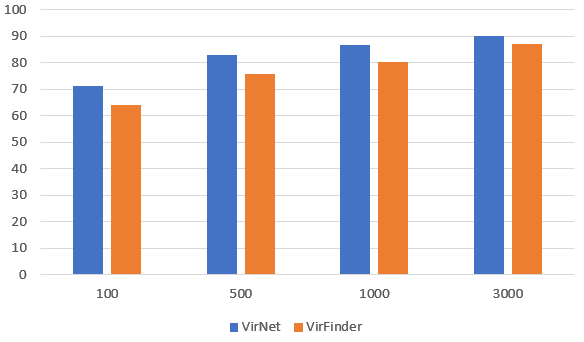
\includegraphics[width=\columnwidth]{Pictures/accuracy_graph.PNG}
	\caption{VirNet vs VirFinder Accuracy}
	\label{fig:accuracy_graph}
\end{figure}


\begin{figure}[!htbp]
	\centering
	\begin{subfigure}{0.5\textwidth}
		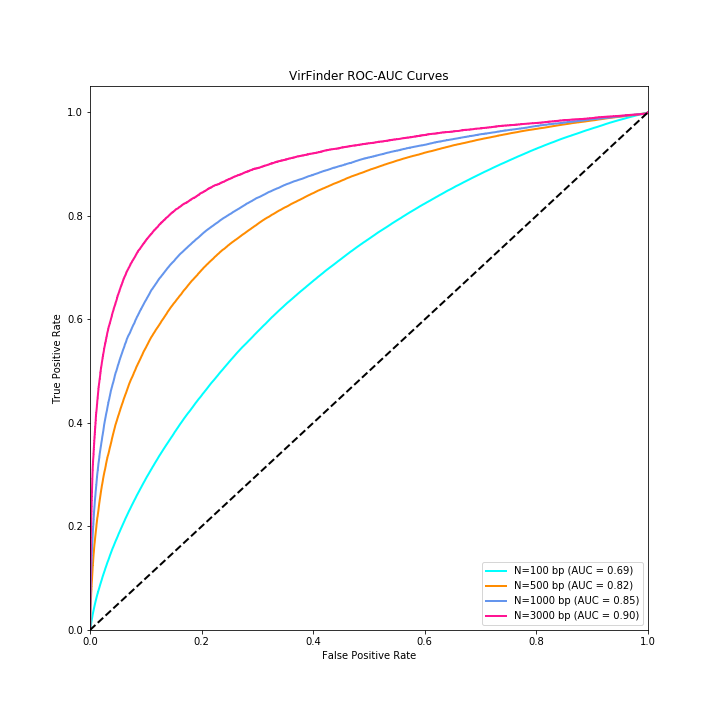
\includegraphics[width=\linewidth]{Pictures/roc_auc.png}
		\caption{VirFinder with generated fragments} 
		\label{fig:roc_auc_virfindera}
	\end{subfigure}
	\begin{subfigure}{0.5\textwidth}
		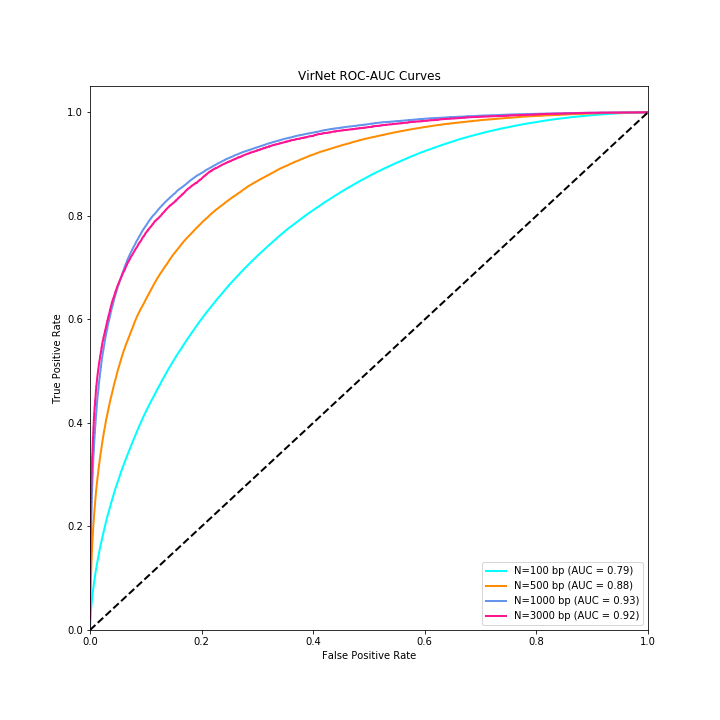
\includegraphics[width=\linewidth]{Pictures/virnet_roc_auc.png}
		\caption{VirNet with generated fragments} 
		\label{fig:roc_auc_virneta}
	\end{subfigure}
	\caption{ROC-AUC curves on fragments} 
	\label{fig:roc_auc_virfinder}
\end{figure}


\begin{figure}[!htbp]
	\centering	
	\begin{subfigure}{0.5\textwidth}
	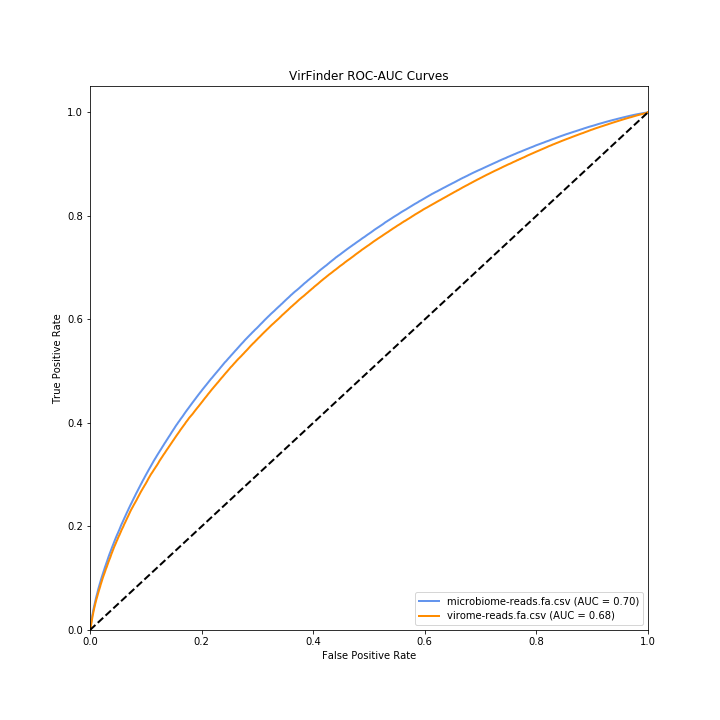
\includegraphics[width=\linewidth]{Pictures/roc_auc_simulated.png}
	\caption{VirFinder with simulated genomes} 
	\label{fig:roc_auc_virfinderb}
\end{subfigure}
\begin{subfigure}{0.5\textwidth}
	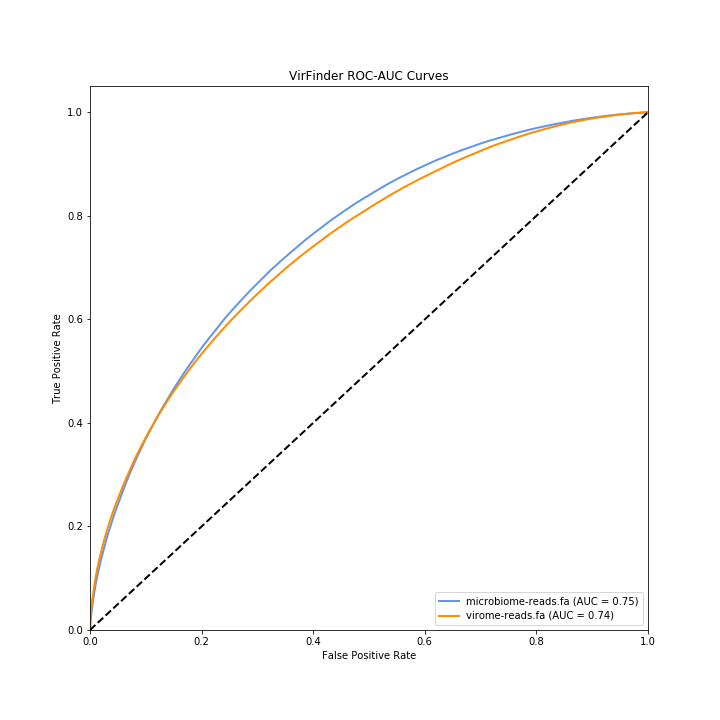
\includegraphics[width=\linewidth]{Pictures/virnet_roc_auc_simulated.png}
	\caption{VirNet with simulated genomes} 
	\label{fig:roc_auc_virnetb}

\end{subfigure}
		\caption{ROC-AUC curves on simulated metagenomes} 
		\label{fig:roc_auc_virfinder2}
\end{figure}

\begin{table}[!htbp]
	\centering
	\begin{tabular}{||l l l l l l l||} 
		Metagenome &	\multicolumn{2}{l}{Accuracy} & \multicolumn{2}{l}{Avg. Precision} & \multicolumn{2}{l}{Avg. Recall}\\ [0.5ex] 
		& VirNet & VirFinder & VirNet & VirFinder & VirNet & VirFinder \\
		\hline\hline
		Virome & 71.3\% &	62.77\%	& 0.71 & 0.63 & 0.72 & 0.62 \\
		Microbiome &	72.14\% & 64.49\% &	0.73 & 0.65 & 0.73 & 0.64 \\ [1ex]
	\end{tabular}
	\caption{Simulated Metagenomes Results}
	\label{table:virfinder_results_simulated}
\end{table}

\subsection{Results for real data}
we applied the tool on two real data with accession numbers SRR648314, SRX995836\_1 and SRX995836\_2. Table \ref{table:virnet_results_real} shows that our tool could able work on the real metagenomic data. 

\begin{table}[]
	\centering
	\begin{tabular}{||llll||}
		& SRR648314 & SRR1974517/1 & SRR1974517/2 \\
		\hline\hline
		Viral     & 39447     & 579697       & 590869       \\
		Non Viral & 20866     & 1055975      & 1044803      \\
		Total     & 60313     & 1635672      & 1635672     
	\end{tabular}
	\caption{VirNet results on real data}
	\label{table:virnet_results_real}
\end{table}

\subsection{VirNet processing speed}
Using GPUs is an advantage for our tool and make it very fast and scalable in processing massive amount of metagenomic reads simultaneously. The training process is around 5 hours with 2 million reads, while the prediction process is around 30 seconds on 1 million reads using Nvidia GeForce GTX 1080 Ti. On the other hand, VirFinder processing the reads on a single CPU less than VirNet by around 82 times. We can avoid that by using parallel CPU threads for VirFinder but in case you want to retrain it with new data, it will take a couple of days.

